El presente capítulo introduce la problemática abordada en este trabajo, describe la propuesta de solución, justifica su pertinencia y establece los objetivos que guían la investigación. Se presenta el contexto de la inteligencia artificial aplicada a videojuegos, se identifica la pregunta central sobre la viabilidad del aprendizaje en tiempo real bajo restricciones de ejecución local y se plantea la necesidad de un entorno experimental que permita cuantificar dicha viabilidad con evidencia empírica.

\section{Presentación del área y su problemática}

\subsection{Contexto de aplicación del proyecto}
El presente proyecto de titulación no se realiza en convenio con una empresa o institución específica, sino que se enmarca dentro del ámbito de la investigación aplicada en inteligencia artificial y desarrollo de videojuegos. En particular, se enfoca en la evaluación experimental del rendimiento y desempeño del aprendizaje de agentes de IA en un entorno de videojuego ejecutado en hardware local, con el objetivo de cuantificar la viabilidad de distintos paradigmas de aprendizaje bajo restricciones de ejecución offline.

\subsection{Presentación de los procesos del ámbito del proyecto}

En los últimos años, el desarrollo de inteligencias artificiales (IA) aplicadas a videojuegos ha evolucionado desde modelos deterministas ---como las máquinas de estados finitos (FSM) o los árboles de decisión--- hacia arquitecturas basadas en \textit{Machine Learning} (ML) y \textit{Reinforcement Learning} (RL). Estas tecnologías permiten entrenar agentes con comportamientos más complejos y variados durante la fase de desarrollo, aunque en la mayoría de los casos los modelos se despliegan como políticas fijas en el producto final.

Una pregunta natural que surge de estos avances es: ¿puede una IA aprender en tiempo real del jugador, adaptándose durante la partida sin depender de servidores externos ni de la nube? Esta posibilidad tendría implicaciones significativas para la industria del videojuego, ya que permitiría crear experiencias que se adapten al estilo de cada jugador utilizando exclusivamente los recursos del hardware local. Además, su aplicabilidad se extendería a otros dominios donde se requiera adaptación en tiempo real con recursos limitados, como sistemas de recomendación embebidos o asistentes interactivos.

Sin embargo, los enfoques actuales de entrenamiento de modelos de ML suelen realizarse en entornos de desarrollo separados del producto final, empleando plataformas como Google Colab, Hugging Face Spaces o Unity ML-Agents \cite{juliani2018mlagents}, que frecuentemente requieren conectividad constante y acceso a GPU de alto rendimiento. Esta práctica indica que el entrenamiento ---tal como se implementa actualmente--- está pensado para la fase de desarrollo, no para ejecutarse dentro del juego durante una sesión con el jugador. No obstante, la viabilidad real de entrenar modelos en tiempo real con los datos que un jugador genera durante una sesión no ha sido cuantificada experimentalmente.

El ciclo convencional de IA en la industria del videojuego presenta las siguientes características:

\begin{itemize}
    \item \textbf{Separación entre entrenamiento y despliegue:} los modelos se entrenan en entornos externos y se integran como políticas fijas en el juego final.
    \item \textbf{Dependencia de volúmenes masivos de datos:} los paradigmas de aprendizaje automático requieren miles a millones de episodios para converger.
    \item \textbf{Ausencia de cuantificación:} no se ha medido experimentalmente cuántos datos genera un jugador humano en una sesión y cómo se compara con lo requerido por los paradigmas de aprendizaje.
\end{itemize}

El presente proyecto busca abordar esta brecha mediante la creación de un entorno experimental que permita cuantificar el costo real de entrenamiento de distintos paradigmas de IA, contrastar ese costo con los datos disponibles en una sesión de juego real contra un jugador humano, y explorar alternativas de adaptación que sean viables bajo restricciones de ejecución local. Se busca determinar si el aprendizaje en tiempo real es factible, o si existen alternativas prácticas ---como la adaptación por selección de especialistas pre-entrenados--- que logren el mismo objetivo sin requerir entrenamiento durante la partida.

En este proyecto se opta por un videojuego de reglas simples, turnos discretos y estado completamente observable (\textit{Knucklebones}), lo que permite aislar el comportamiento de la inteligencia artificial, reducir ruido experimental y facilitar mediciones reproducibles.

\subsubsection{Evolución del alcance del proyecto}

El proyecto fue concebido inicialmente con un enfoque orientado a un videojuego en primera persona (\textit{First Person Shooter}, FPS), dado que este género representa un escenario atractivo para evaluar toma de decisiones y adaptación del comportamiento en agentes controlados por IA. Sin embargo, durante el desarrollo se identificaron dos factores determinantes para reformular el alcance:

\begin{itemize}
    \item \textbf{Complejidad de implementación y riesgo técnico:} un FPS introduce múltiples variables simultáneas (física, navegación, percepción parcial, sincronización en tiempo real, animaciones, balance de combate y diseño de niveles), lo que incrementa el riesgo de que los resultados experimentales se vean afectados por aspectos ajenos al objetivo principal de la investigación.
    \item \textbf{Irrelevancia del género para el objetivo experimental:} el objetivo de este trabajo no es evaluar la calidad audiovisual o el diseño de un género específico, sino estudiar el desempeño, costo computacional y reproducibilidad de distintos enfoques de IA en un entorno de videojuego. Por lo tanto, la naturaleza del entorno debe privilegiar control experimental y medición.
\end{itemize}

En consecuencia, se optó por un entorno de reglas simples, turnos discretos y estado completamente observable (\textit{Knucklebones}). Esta elección permite aislar el problema de decisión, reducir ruido experimental y fortalecer la reproducibilidad de resultados, manteniendo el foco del proyecto en la evaluación del costo de aprendizaje y mecanismos de adaptación bajo restricciones de ejecución local. La Figura~\ref{fig:evolucion_alcance} ilustra esta transición.

\begin{figure}[H]
\centering
\begin{tikzpicture}[
    block/.style={rectangle, draw, rounded corners, minimum height=1.2cm, text width=3.5cm, align=center, font=\small},
    arrow/.style={-{Stealth[length=3mm]}, thick},
]
\node[block, fill=red!15] (fps) {\textbf{Concepto inicial}\\Videojuego FPS\\(alta complejidad)};
\node[block, fill=yellow!20, right=1.5cm of fps] (analisis) {\textbf{Análisis de riesgos}\\Ruido experimental,\\variables no controladas};
\node[block, fill=green!15, right=1.5cm of analisis] (kb) {\textbf{Entorno final}\\Knucklebones\\(control experimental)};

\draw[arrow] (fps) -- (analisis);
\draw[arrow] (analisis) -- (kb);
\end{tikzpicture}
\caption[Evolución del alcance del proyecto]{Evolución del alcance del proyecto: del concepto FPS al entorno controlado Knucklebones.}
\label{fig:evolucion_alcance}
\end{figure}

La Figura~\ref{fig:fps_antiguo} muestra el prototipo FPS original, cuya complejidad motivó la transición hacia un entorno de menor ruido experimental.

\begin{figure}[H]
\centering
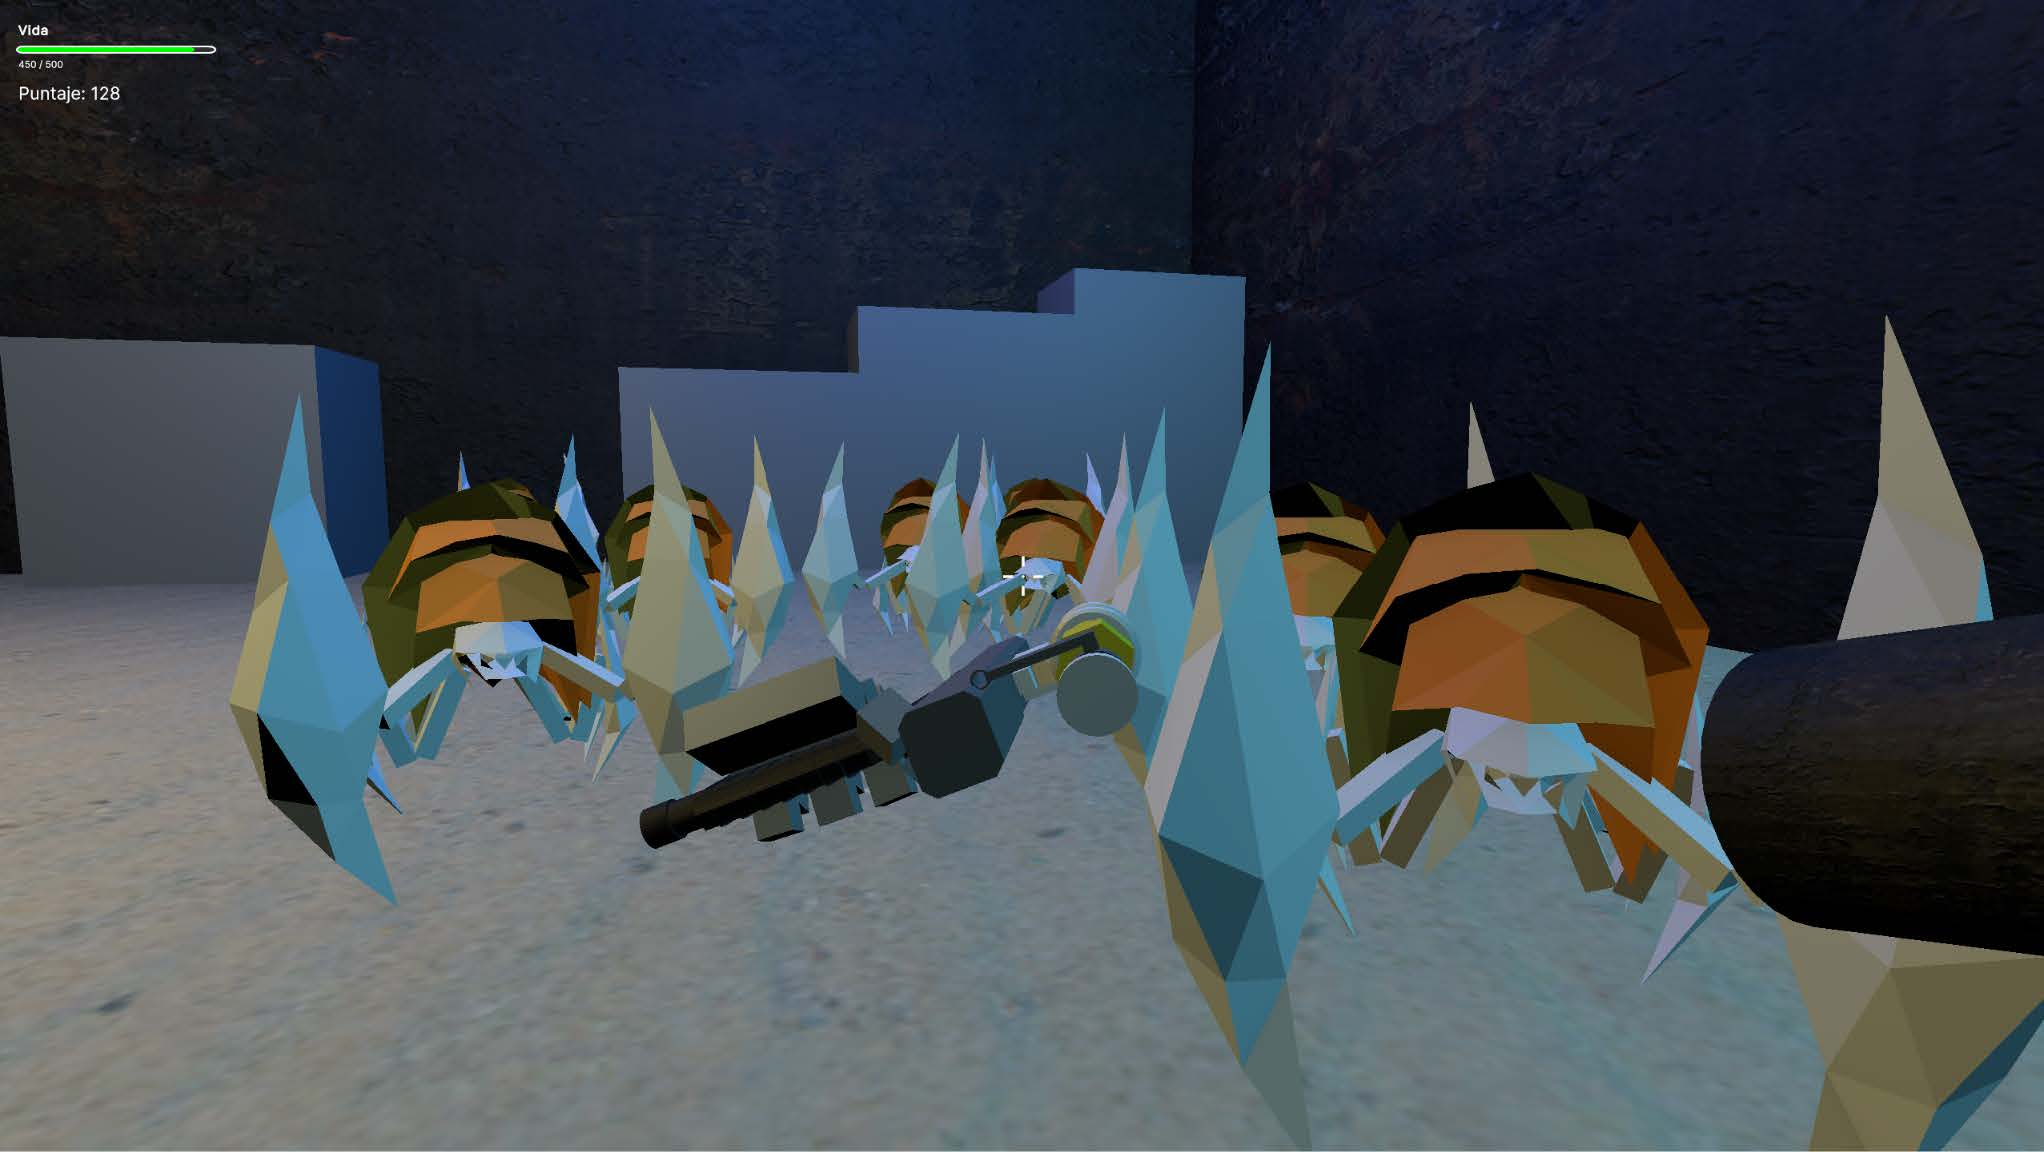
\includegraphics[width=0.7\textwidth]{figures/fpsingame.jpg}
\caption[Prototipo exploratorio FPS]{Prototipo exploratorio inicial del entorno FPS en Unity, desarrollado durante la primera fase del proyecto. Esta versión se utilizó para validar jugabilidad base y la viabilidad de integrar métricas en hardware local, pero fue descartada como entorno experimental principal por su alta complejidad y bajo control metodológico.}
\label{fig:fps_antiguo}
\end{figure}

\subsection{Descripción del Problema}

Actualmente, existe una percepción extendida ---tanto en la industria del videojuego como en la comunidad académica--- de que las inteligencias artificiales en videojuegos pueden o deberían ``aprender en tiempo real'' mientras interactúan con el jugador. Casos recientes como ARC Raiders han sido promocionados sugiriendo que los enemigos exhiben comportamientos emergentes aprendidos durante el gameplay, cuando la evidencia pública disponible indica que los modelos fueron entrenados durante el desarrollo y desplegados como políticas fijas.

Esta percepción genera una brecha entre la expectativa y la realidad técnica. Los paradigmas de aprendizaje automático más utilizados ---aprendizaje por refuerzo, neuroevolución, aprendizaje supervisado--- requieren volúmenes de datos y ciclos de entrenamiento que podrían exceder lo disponible en una sesión de juego contra un jugador humano. Sin embargo, esta brecha no ha sido cuantificada de forma sistemática bajo restricciones de hardware local.

Por otra parte, si bien existen herramientas y entornos para entrenar agentes de IA en videojuegos (como OpenAI Gym \cite{brockman2016openai}, Unity ML-Agents \cite{juliani2018mlagents} o Stable-Baselines3 \cite{raffin2021sb3}), estas están orientadas principalmente al proceso de entrenamiento offline, no a cuantificar la brecha entre los datos requeridos para entrenar y los datos que un jugador humano genera en una sesión real. Esta cuantificación resulta necesaria para determinar la viabilidad del aprendizaje en tiempo real.

El problema central que aborda este proyecto radica en la ausencia de evidencia experimental que cuantifique la viabilidad del aprendizaje de IA en tiempo real bajo restricciones de ejecución local, y en la necesidad de explorar alternativas ---como la adaptación por selección de especialistas pre-entrenados--- que ofrezcan adaptabilidad sin depender de entrenamiento online continuo.

\section{Propuesta de solución}

La propuesta de solución consiste en diseñar e implementar un entorno experimental que permita determinar, con evidencia cuantitativa, si es factible que una inteligencia artificial aprenda en tiempo real del jugador en un videojuego ejecutado en hardware local. Para ello, se construye una plataforma basada en un juego de turnos discretos (\textit{Knucklebones}), donde se entrenan tres paradigmas representativos de IA y se mide rigurosamente el costo de dicho entrenamiento, contrastándolo con los datos que un jugador humano genera en una sesión real.

El proyecto plantea dos líneas complementarias:

\begin{enumerate}
    \item \textbf{Cuantificación de la viabilidad del aprendizaje en tiempo real}: entrenar tres paradigmas de IA (aprendizaje por refuerzo, neuroevolución, aprendizaje supervisado destilado) de forma offline, midiendo los datos requeridos, el tiempo de entrenamiento y los recursos computacionales consumidos. Estos datos permiten evaluar la brecha entre los requisitos de cada paradigma y lo disponible en una sesión de juego real contra un jugador humano, determinando si el aprendizaje en tiempo real es viable o no.
    \item \textbf{Adaptación por selección como alternativa}: dado que la hipótesis inicial sugiere que el aprendizaje en tiempo real podría no ser viable con los paradigmas convencionales, se diseña e implementa un mecanismo de adaptación que no requiera reentrenamiento en tiempo de ejecución, basado en perfilado del oponente (clustering no supervisado) y selección de especialistas pre-entrenados. Este mecanismo se evalúa como alternativa práctica al entrenamiento online continuo.
\end{enumerate}

Para ello, se emplea el motor de desarrollo Unity como entorno de ejecución de reglas, junto con una arquitectura modular diseñada desde el inicio con separación estricta entre el motor del juego (responsable de reglas y transición de estado) y los agentes de IA (responsables exclusivamente de la selección de acciones). Un middleware HTTP/JSON permite la comunicación entre ambas capas. Esta separación modular fue una decisión de diseño planificada, no una limitación descubierta durante el desarrollo.

El sistema incluye instrumentación capaz de registrar métricas tales como latencia de decisión, carga computacional, tiempo de entrenamiento y tamaño de modelo. Estas métricas permiten evaluar de manera objetiva tanto el desempeño de cada enfoque como su costo, determinando su viabilidad bajo restricciones de hardware local.


La ejecución local en hardware convencional garantiza accesibilidad y reduce dependencia de recursos remotos. El diseño modular permite incorporar nuevos agentes o configuraciones experimentales con bajo costo adicional.

\subsection{Separación entre entrenamiento y ejecución}

Desde el diseño inicial del proyecto se estableció una arquitectura modular que separa la lógica del videojuego de los agentes de IA. El videojuego se mantiene como entorno estable que expone estado y recibe acciones, mientras que el entrenamiento se realiza fuera del motor utilizando un entorno equivalente tipo \textit{Gym} \cite{brockman2016openai}. Esta decisión de diseño responde a criterios de reproducibilidad, trazabilidad y eficiencia experimental.

El entorno equivalente permite ejecutar partidas a alta velocidad, generar datasets y entrenar modelos con mayor eficiencia, manteniendo consistencia con las reglas del juego y conservando la ejecución en hardware local. Esta separación no contradice el objetivo de evaluar la viabilidad del aprendizaje en tiempo real; por el contrario, permite medirla de forma rigurosa: si el entrenamiento offline ---en condiciones óptimas de velocidad y volumen de datos--- ya requiere órdenes de magnitud más datos de los disponibles en una sesión real, el entrenamiento en tiempo real durante la partida resulta inviable.

De esta manera, el sistema mantiene equivalencia funcional entre el entorno de entrenamiento y el entorno de evaluación, garantizando la validez experimental de los resultados obtenidos.

\section{Justificación de la propuesta}

El desarrollo de este proyecto se justifica por la necesidad de responder, con evidencia experimental, a una pregunta que la industria del videojuego y la comunidad académica asumen implícitamente pero no han cuantificado: ¿es viable que una inteligencia artificial aprenda en tiempo real dentro de un videojuego ejecutado en hardware local?

\textbf{Desde un punto de vista técnico}, la propuesta aborda esta pregunta mediante la medición rigurosa del costo de entrenamiento de tres paradigmas representativos (aprendizaje por refuerzo, neuroevolución, aprendizaje supervisado), cuantificando los datos, el tiempo y los recursos requeridos, y contrastándolos con lo disponible en una sesión real. La separación modular entre juego y agentes permite aislar el rendimiento del aprendizaje de factores externos, y el diseño del sistema habilita la evaluación de alternativas como la adaptación por selección.

\textbf{En términos de reproducibilidad}, la evaluación y el entrenamiento se realizan localmente en hardware doméstico, sin requerir infraestructura externa. Esto garantiza que los resultados puedan ser replicados por otros investigadores con recursos similares y elimina dependencias de servicios en la nube.

\textbf{Funcionalmente}, el sistema incluye instrumentación integrada que registra no solo el desempeño del agente durante el juego (winrate, latencia), sino también el costo del proceso de aprendizaje (tiempo de entrenamiento, datos requeridos, tamaño de modelo). Esta doble medición permite un análisis de viabilidad fundamentado en evidencia.

\textbf{Desde una perspectiva de investigación}, este proyecto contribuye con evidencia cuantitativa sobre una pregunta que, si bien es relevante tanto para la industria del videojuego como para cualquier dominio que requiera adaptación en tiempo real con recursos limitados, ha sido poco abordada de forma experimental: ¿cuánto cuesta realmente que una IA aprenda, y es posible hacerlo con los datos que genera un usuario en una sesión real?

\section{Objetivos}

\subsection{Objetivo General}

Evaluar el rendimiento y desempeño del aprendizaje de distintas inteligencias artificiales en un entorno de videojuego ejecutado completamente offline, cuantificando la brecha entre los requisitos de entrenamiento de tres paradigmas representativos y los datos disponibles en una sesión real contra un jugador humano, con el fin de determinar la viabilidad del aprendizaje en tiempo real y evaluar la adaptación por selección de especialistas pre-entrenados como alternativa práctica, sin depender de infraestructura en la nube.

\section{Alcance y limitaciones}

El trabajo abarca los siguientes elementos:

\begin{itemize}
    \item Diseño e implementación de una arquitectura modular que separa el videojuego de los agentes de IA.
    \item Entrenamiento de especialistas en tres paradigmas: PPO (aprendizaje por refuerzo), NEAT (neuroevolución) y DT (destilación por \textit{Behavior Cloning}).
    \item Medición del costo de entrenamiento de cada paradigma (datos, tiempo, recursos).
    \item Análisis de la brecha entre los datos requeridos y los disponibles en una sesión contra un jugador humano.
    \item Implementación de un mecanismo de adaptación por selección (KMeans + response table + especialistas).
    \item Integración del sistema completo en Unity mediante middleware HTTP/JSON.
\end{itemize}

Como limitaciones deliberadas:

\begin{itemize}
    \item No se implementa entrenamiento online completo dentro del motor del juego. Los resultados documentan cuantitativamente por qué dicho entrenamiento no es viable con los paradigmas evaluados.
    \item La estimación de datos disponibles en una sesión humana (10--100 partidas) es un supuesto operativo derivado de observación práctica, no un estudio formal de comportamiento de usuario.
    \item Los oponentes de entrenamiento y evaluación son heurísticos diseñados, no jugadores humanos reales.
    \item El entorno experimental es un juego de reglas simples (Knucklebones); la generalización a dominios más complejos queda como trabajo futuro.
\end{itemize}

\subsection{Objetivos Específicos}
\begin{itemize}
    \item Diseñar una arquitectura modular que permita incorporar y evaluar diferentes enfoques de inteligencia artificial sin modificar las reglas del videojuego.
    \item Implementar un prototipo funcional basado en un videojuego de turnos discretos que opere como plataforma de prueba para la ejecución y evaluación reproducible de agentes.
    \item Entrenar y evaluar tres paradigmas de aprendizaje ---aprendizaje por refuerzo (PPO), neuroevolución (NEAT) y aprendizaje supervisado destilado (DT)--- midiendo el costo de entrenamiento en términos de datos requeridos, tiempo y recursos computacionales.
    \item Cuantificar la brecha entre los requisitos de entrenamiento de cada paradigma y los datos disponibles en una sesión real contra un jugador humano, para determinar la viabilidad del aprendizaje en tiempo real.
    \item Implementar y evaluar un mecanismo de adaptación por selección de especialistas pre-entrenados como alternativa al entrenamiento online continuo.
    \item Integrar los agentes en el videojuego Unity mediante un middleware desacoplado, verificando la viabilidad operativa del sistema completo.
\end{itemize}

\subsection{Descripción de actividades}

\begin{itemize}

    \item \textbf{Diseñar una arquitectura modular para agentes intercambiables.}
    \begin{itemize}
        \item Diseño de la estructura modular del sistema y definición de interfaz estado/acción.
        \item Elaboración de esquemas lógicos y diagramas de componentes.
        \item Definición de flujos para integración de agentes y centralización de extracción de características.
    \end{itemize}

    \item \textbf{Desarrollar el prototipo de videojuego como entorno de evaluación.}
    \begin{itemize}
        \item Construcción del entorno base del juego seleccionado.
        \item Implementación del protocolo de observación por turno y aplicación de acciones.
        \item Aseguramiento de condiciones de control experimental (semillas, registro estructurado).
    \end{itemize}

    \item \textbf{Entrenar y medir el costo de aprendizaje de cada paradigma.}
    \begin{itemize}
        \item Entrenamiento de especialistas PPO mediante aprendizaje por refuerzo con entorno acelerado.
        \item Entrenamiento de especialistas NEAT mediante neuroevolución con evaluación multi-seed.
        \item Destilación de PPO a árboles de decisión mediante \textit{Behavior Cloning}.
        \item Registro de datos requeridos, tiempo de entrenamiento y recursos computacionales por cada paradigma.
    \end{itemize}

    \item \textbf{Cuantificar la brecha de viabilidad para entrenamiento en tiempo real.}
    \begin{itemize}
        \item Estimación de los datos disponibles en una sesión real contra un jugador humano.
        \item Cálculo de la relación entre datos requeridos y datos disponibles por paradigma.
        \item Análisis de convergencia con datos limitados (evidencia de entrenamiento insuficiente).
    \end{itemize}

    \item \textbf{Implementar y evaluar el mecanismo de adaptación por selección.}
    \begin{itemize}
        \item Entrenamiento de perfilador KMeans con datos de oponentes heurísticos.
        \item Construcción de tablas de respuesta por evaluación de especialistas por cluster.
        \item Evaluación comparativa del sistema adaptativo frente a generalistas fijos (\textit{ablation study}).
    \end{itemize}

    \item \textbf{Integrar el sistema completo en el videojuego Unity.}
    \begin{itemize}
        \item Implementación de middleware HTTP/JSON para comunicación Unity--Python.
        \item Verificación de equivalencia funcional entre entorno de simulación y motor de juego.
        \item Medición de latencia operativa del sistema integrado.
    \end{itemize}

\end{itemize}

\section{Descripción de los Aspectos Fundamentales de la Metodología Utilizada}

La presente investigación se enmarcó dentro del paradigma de la investigación aplicada, combinando elementos de análisis experimental, diseño iterativo de software y evaluación comparativa. Debido a la naturaleza técnica del proyecto, que implicó implementar un entorno de evaluación reproducible, instrumentado y controlado para medir de forma cuantificable el comportamiento y el costo computacional de agentes de IA bajo condiciones homogéneas, se adoptó una metodología de carácter evolutivo y orientada a prototipos.

El enfoque metodológico se fundamentó en tres pilares principales:

\begin{itemize}
    \item \textbf{Investigación exploratoria y revisión técnica:} permitió comprender el estado actual de las tecnologías involucradas, incluyendo IA para videojuegos, modularidad de software, instrumentación y limitaciones de hardware local.
    \item \textbf{Desarrollo incremental de prototipos:} el videojuego y los módulos del sistema fueron construidos de manera progresiva, incorporando funcionalidades esenciales en ciclos iterativos. Este enfoque facilitó la validación temprana de componentes, redujo riesgos asociados a la complejidad del sistema y permitió evaluar continuamente la factibilidad técnica del proyecto.
    \item \textbf{Experimentación y análisis de rendimiento:} los enfoques de IA fueron evaluados mediante métricas cuantitativas, incluyendo latencia de decisión, uso de CPU/memoria, estabilidad y métricas de desempeño dentro del juego. Esta fase permitió comparar enfoques bajo condiciones homogéneas y completamente offline.
\end{itemize}

La elección de una metodología evolutiva respondió a la incertidumbre inherente al desarrollo de sistemas de IA y al nivel de riesgo técnico asociado a integración, medición y control experimental. Este enfoque permitió ajustar el diseño del sistema de forma continua y corregir desviaciones durante el avance de la investigación.

En la primera etapa se desarrolló un levantamiento del marco tecnológico y conceptual. Luego se diseñó e implementó una arquitectura modular que soporta la integración de agentes y registro de métricas. Posteriormente, se construyó el prototipo funcional como plataforma de pruebas, sobre el cual se integraron y evaluaron distintos enfoques de IA. Finalmente, se realizó un análisis comparativo de resultados con el fin de determinar la factibilidad técnica y operativa de los enfoques evaluados en un entorno de videojuego ejecutado completamente en hardware local.

De esta manera, la metodología seleccionada garantizó una progresión controlada del proyecto, favoreció la validación temprana de hipótesis y aseguró que los objetivos planteados pudieran ser alcanzados mediante un proceso sistemático, reproducible y fundamentado en evidencia experimental.

\section{Composición del informe}

El presente trabajo se encuentra dividido en seis capítulos. A continuación se describe brevemente el contenido de cada uno de ellos.

\begin{enumerate}
    \item \textbf{Introducción:} presentación del problema, objetivos, alcance y metodología general del trabajo.
    \item \textbf{Bases Teóricas:} fundamentos sobre IA en videojuegos, aprendizaje automático, distinción entre aprendizaje online y adaptación por selección, costos de entrenamiento y reproducibilidad experimental.
    \item \textbf{Estado del Arte:} revisión de enfoques existentes en la industria y la academia, con énfasis en la viabilidad del aprendizaje en tiempo real y las prácticas de adaptación utilizadas.
    \item \textbf{Desarrollo del trabajo:} diseño e implementación de la plataforma, arquitectura modular, instrumentación, flujo experimental y criterios de viabilidad para entrenamiento en tiempo real.
    \item \textbf{Resultados:} medición de costos de aprendizaje, análisis de brecha de datos, evaluación de sistemas adaptativos, discusión de viabilidad y comparación de paradigmas.
    \item \textbf{Conclusiones:} síntesis de hallazgos sobre viabilidad del aprendizaje, validación de la adaptación por selección y proyecciones.
\end{enumerate}

Además, al final del informe se adjuntan las referencias bibliográficas utilizadas en el proceso de investigación.
\vfill